\scanpage{27}
\figure{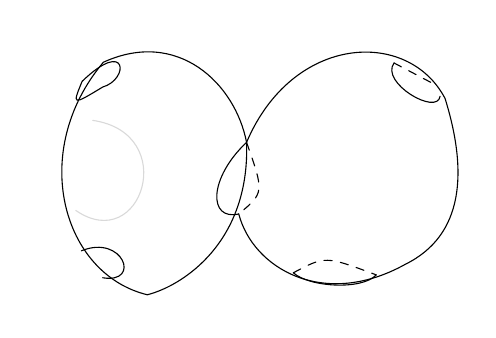
\begin{tikzpicture}[x=.009cm,y=-.009cm,line cap=round]
\draw (-140,-95) .. controls (-35,-143) and (46,-65) .. (62,18) .. controls (67,158) and (-27,220) .. (-78,233) .. controls (-198,204) and (-246,31) .. (-140,-95);
\draw (62,18) .. controls (127,-135) and (290,-143) .. (342,-44) .. controls (374,59) and (369,149) .. (286,190) .. controls (171,254) and (71,196) .. (51,119);
\draw (62,18) .. controls (8,69) and (8,129) .. (51,119);
\draw[dashed] (62,18) .. controls (87,89) .. (51,119);
\draw (-170,-68) .. controls (-106,-130) and (-103,-71) .. (-141,-60) .. controls (-184,-34) .. (-170,-68);
\draw (-171,171) .. controls (-112,147) and (-86,218) .. (-141,209);
\draw (270,-94) .. controls (250,-66) and (331,-19) .. (335,-47);
\draw[dashed] (270,-94)--(325,-65);
\draw (128,202) .. controls (150,222) and (224,227) .. (245,205);
\draw[dashed] (128,202) .. controls (173,178) .. (245,205);
\draw[gray!30] (-155,-13) .. controls (-31,5) and (-86,178) .. (-179,114);
\end{tikzpicture}}
\diagram{\begin{tikzcd}[column sep=large]
\left.\begin{array}{l}
4\text{ hexagones}\\16\ \unsure{\text{côtés}|\text{arêtes}}\\10\text{ sommets}
\end{array}\right\}
\arrow[r,Rightarrow] &
\begin{array}{l}8\text{ hexagones}\\\unsure{82|32}\text{ arêtes}\\16\text{ sommets}\end{array}
\\
\begin{array}{l}(\text{dont }4\text{ ramifiés})\\\text{d'ordre}\end{array}&
\end{tikzcd}}
\begin{gather*}
2\text{ hexag.}\\9\text{ arêtes}\\6\text{ sommets}
\end{gather*}
\figure{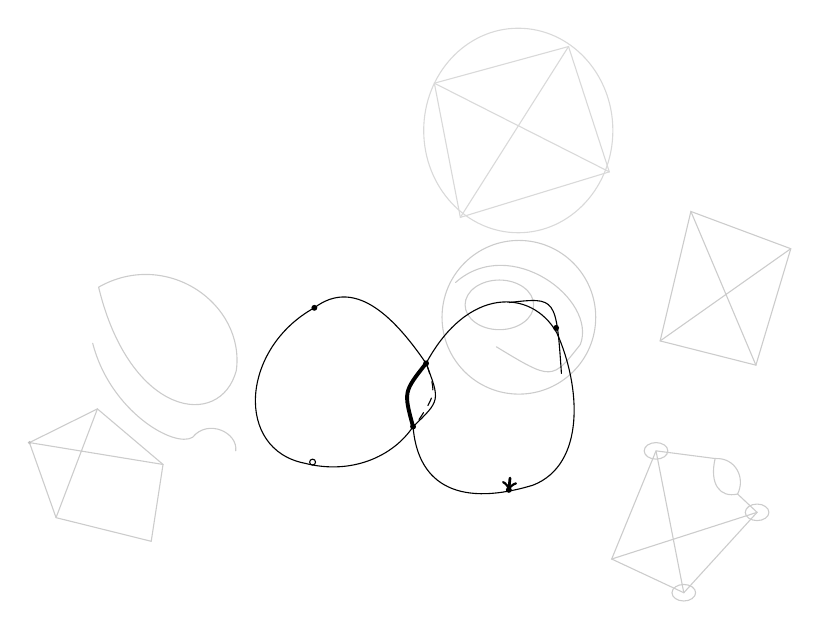
\begin{tikzpicture}[x=.0075cm,y=-.0075cm,line cap=round]
\draw[gray!30] (320,-440) ellipse (160 and 173);
\draw[gray!30] (178,-520)--(405,-582)--(474,-370)--(222,-293)--cycle;
\draw[gray!30] (178,-520)--(474,-370) (405,-582)--(222,-293);
\draw[gray!40] (-390,-175) .. controls (-275,-240) and (-142,-147) .. (-157,-34) .. controls (-184,67) and (-337,45) .. (-390,-175);
\draw[gray!40] (-400,-80) .. controls (-370,36) and (-261,98) .. (-231,79) .. controls (-205,47) and (-154,71) .. (-158,102);
\draw[gray!40] (-507,88)--(-392,31)--(-281,125)--(-301,255)--(-462,215)--cycle;
\draw[gray!40] (-507,88)--(-281,125) (-392,31)--(-462,215);
\fill[gray!50] (-507,88) circle (3);
\draw[gray!40] (321,-124) circle (130);
\draw[gray!40] (214,-183) .. controls (307,-265) and (454,-154) .. (425,-78) .. controls (377,-17) .. (283,-74);
\draw[gray!40] (288,-145) ellipse (58 and 42);
\draw[gray!40] (612,-303)--(781,-240)--(722,-43)--(560,-84)--cycle;
\draw[gray!40] (612,-303)--(722,-43) (781,-240)--(560,-84);
\draw[gray!40] (653,115) .. controls (687,113) and (705,147) .. (691,175) .. controls (661,182) and (643,158) .. (653,115);
\draw[gray!40] (553,102)--(653,115) (691,175)--(724,206)--(600,342)--(478,285)--(553,102);
\draw[gray!40] (553,102)--(600,342) (478,285)--(724,206);
\foreach \x/\y in {553/102,724/206,600/342}{\draw[gray!40] (\x,\y) ellipse (20 and 14);}
\draw (-25,-140) .. controls (-150,-71) and (-160,100) .. (-41,123) .. controls (37,143) and (108,112) .. (142,61);
\draw (-25,-140) .. controls (41,-190) and (106,-131) .. (164,-46);
\draw (164,-46) .. controls (234,-176) and (342,-173) .. (385,-98) .. controls (426,-7) and (434,125) .. (345,160) .. controls (209,201) and (149,151) .. (142,61);
\draw[line width=1.4pt] (164,-46) .. controls (126,2) .. (142,61);
\draw (164,-46) .. controls (188,17) .. (142,61);
\draw[dashed] (166,-42) .. controls (181,6) .. (146,58);
\draw (305,-149) .. controls (384,-158) .. (393,-29);
\foreach \x/\y in {-25/-140,164/-46,142/61,384/-106,304/168}{\fill (\x,\y) circle (5);}
\draw (-28,121) circle (5);
\draw[->,line width=1pt] (306,148)--(304,168);
\end{tikzpicture}}% crop-candidate: scan 27
\diagram{\begin{tikzcd}[column sep=large]
\left.\begin{array}{l}
6\text{ sommets}\\(\text{dont }4\text{ ramifiés})\\
8\text{ arêtes}\\
4\ \deleted{\text{triangles}}\inserted{\text{carrés}}
\end{array}\right\}
\arrow[r,Rightarrow]&
\begin{array}{l}
8\text{ sommets}\\\text{d'ordre }4\\16\text{ arêtes}\\
8\ \deleted{\text{triangles}}\inserted{\text{carrés}}
\end{array}\arrow[d,bend right=20]\\
&\deleted{\unsure{1|4}\times4\text{ d'ordre}}\ 4
\end{tikzcd}}
\figure{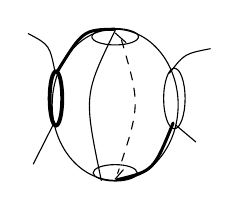
\begin{tikzpicture}[x=.8cm,y=.8cm,line cap=round]
\draw (0,0) ellipse (1 and 1.2);
\draw (0,1.08) ellipse (.37 and .13) (0,-1.08) ellipse (.35 and .13);
\draw[line width=1.4pt] (-.94,.1) ellipse (.1 and .43);
\draw (.94,.1) ellipse (.17 and .48);
\draw (.86,.5) .. controls (1.1,.81) .. (1.51,.89) (.96,-.32)--(1.28,-.59);
\draw (-.95,.5)..controls (-1.04,.95)..(-1.38,1.13) (-.97,-.29)--(-1.3,-.94);
\draw (0,1.18)..controls (-.5,.15)..(-.22,-1.2);
\draw[dashed] (.1,1.03)..controls (.4,0)..(.04,-1.09);
\draw[line width=1.1pt] (-.93,.51)..controls (-.51,1.19)..(0,1.2) (.92,-.29)..controls (.61,-1.05)..(.03,-1.19);
\draw (0,1.14)--(.17,.99) (0,-1.18)--(.13,-1.03);
\end{tikzpicture}}
\figure{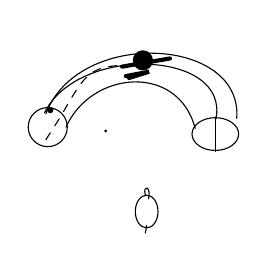
\begin{tikzpicture}[x=.8cm,y=.8cm,line cap=round]
\draw (-1.4,-.1) .. controls (-.89,1.26) and (1.73,1.13) .. (1.63,-.17);
\draw (-1.42,-.08) .. controls (-.89,1) and (1.52,.92) .. (1.3,-.18);
\draw (-1.08,-.31) .. controls (-.68,.59) and (.7,.71) .. (.97,-.33);
\draw (-1.37,-.31) circle (.31) (1.29,-.42) ellipse (.37 and .26);
\draw (1.29,-.15)--(1.29,-.7);
\draw[dashed] (-1.4,-.51)--(-1.17,-.15)..controls (-.7,.67)..(.22,.68);
\fill (.14,.75) circle (.16);
\draw[line width=1.5pt] (-.19,.65)--(.57,.78) (-.08,.47)--(.24,.57)--(-.13,.5);
\fill (-1.33,-.04) circle (.05);
\fill (-.45,-.37) circle (.025);
\draw (.2,-1.65) ellipse (.18 and .26);
\draw (.2,-1.87)--(.18,-1.99) (.18,-1.39) .. controls (.13,-1.22) and (.28,-1.24) .. (.23,-1.45);
\end{tikzpicture}}
\margin{Justine}
\margin{26}
